\documentclass[9pt]{beamer}

\usepackage{amsmath,amsthm,amssymb} %fuer math. Formeln
\usepackage{graphicx} %fuer Bilder
\usepackage{color} %fuer farbigen Text
\usepackage{listings}
\lstset{
  language=XML,
	backgroundcolor = \color{lightgray},
  basicstyle=\tiny,
columns=fullflexible
}

\usepackage[utf8]{inputenc}
\DeclareUnicodeCharacter{00A0}{ }

\usetheme{Berlin}  % Vorlage, welche das Aussehen der Praesentation festlegt-andere Alternativen: AnnArbor, Bergen,...
\usecolortheme{orchid} % Vorlage, welche das Farblayout der Praesentation festlegt -andere Alternativen: lily, beetle,...
\author{Iryna Repinetska, Chris Roeseler}
\title{BIBO - Bibliotheks Bot}
\institute{Institut f\"ur Informatik Humboldt-Universit\"at zu Berlin}
\date{\today} 



\begin{document}

\begin{frame}% Beginne eine Slide 
  \titlepage % Inhalt (In diesem Fall die Titelseite)
\end{frame} % Beende eine Slide

\section{Spezifikationen von Bibo}
\begin{frame}
  Bibo soll ein persönlicher Bibliothekar werden und folgende Funktionalitäten bieten:
\begin{itemize}
\item Im Gespräch das Thema festlegen
\item Alle Bücher eines Themas auflisten
\item Auswahl im Gespräch einschränken
\item Position und Verfügbarkeit in der Bibliothek ausgeben
\end{itemize}
\end{frame}

\section{Dialog}
\begin{frame}
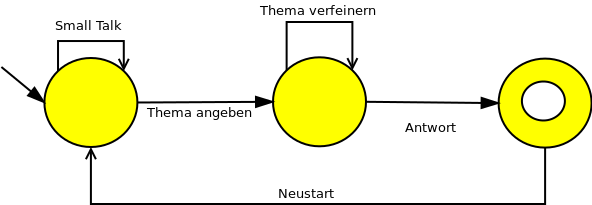
\includegraphics[width=\textwidth]{Diagram1.png} %70% der Textbreite
\end{frame}

\section{Datenfluss}
\begin{frame}
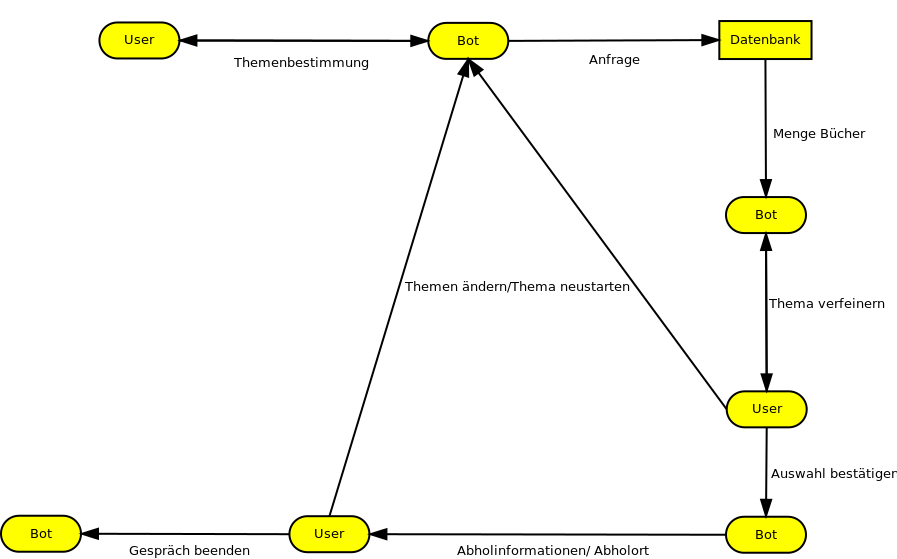
\includegraphics[width=\textwidth]{Diagram2.png} %70% der Textbreite
\end{frame}


\section{Komponentenarchitektur}
\begin{frame}
  \begin{itemize}
    \item AIML
    \begin{itemize}
      \item Wordnet
    \end{itemize}
    \item Exlibris PRIMO
    \item Python
    \item easyrec
  \end{itemize}
\end{frame}

\section{Implementierungskonzepte}
\begin{frame}
  \begin{itemize}
    \item Korpus: Python
    \begin{itemize}
      \item Verbindet die API's und AIML Interface
    \end{itemize}
    \item AIML - simple Gesprächsmuster
    \item Exlibris PRIMO
    \begin{itemize}
      \item Stellt Zugriff auf Bibliotheksdatenbank 
      \item Ermöglicht Auflisten, Fundort, Leihstatus
    \end{itemize}
  \end{itemize}
\end{frame}

\end{document}
